\section{去除电磁场仿真端口效应}
理想无限长传输线各处均匀,实际电磁场仿真中由于硬件以及时间限制,实际电磁场仿真的模型长度有限。
由于电磁场仿真中端口和模型信号线本身的不连续性导致信号线上电场磁场分布不均匀。图 \ref{fig:e_field}中为
一200um长CPW的电场分布图,从图中可以看出模型电场中间部分分布均匀,而两端口处分布不均匀。
理想情况下,不同长度的CPW计算得到其单位长度RLGC值应该是相同的,由于端口效应的影响不同
长度的CPW计算得到其单位长度RL值如图\ref{fig:unit_RL2}所示,从图中可以看出其不同长度的CPW计算得到其
单位长度RL值与CPW模型长度相关。
\begin{figure}[htb]
  \centering
  \includegraphics[width=12 cm]{E_field.png}
  \caption{200um长CPW的电场分布图} \label{fig:e_field}
\end{figure}

\begin{figure}[htb]
\centering
  % Requires \usepackage{graphicx}
  \subfloat[单位长度R]{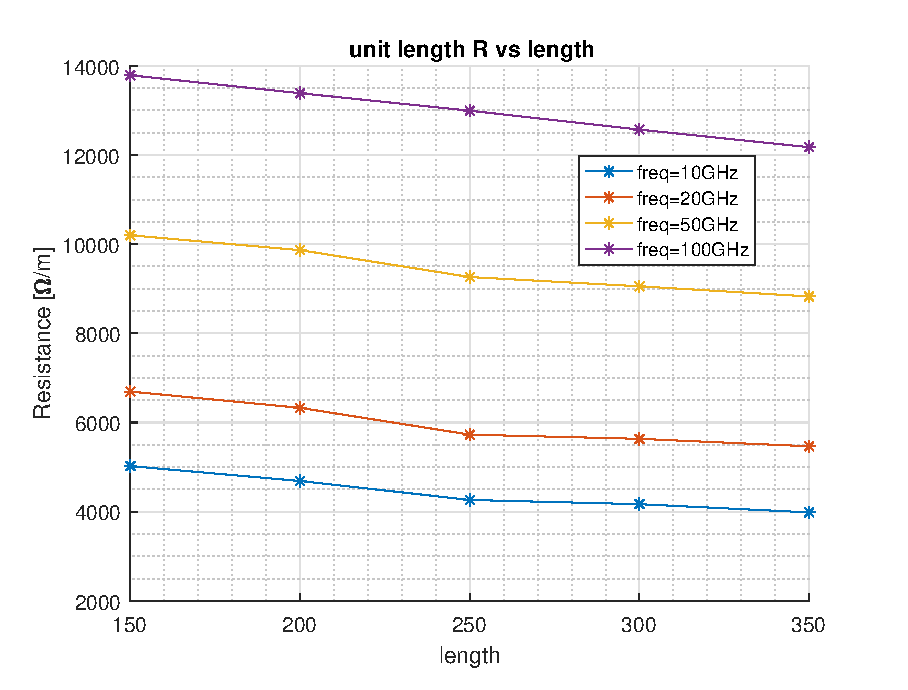
\includegraphics[width=7cm]{R_unit_len.eps}\label{fig:unit_R}}
 \hspace{0.1cm}
 %\qquad
  \subfloat[单位长度L]{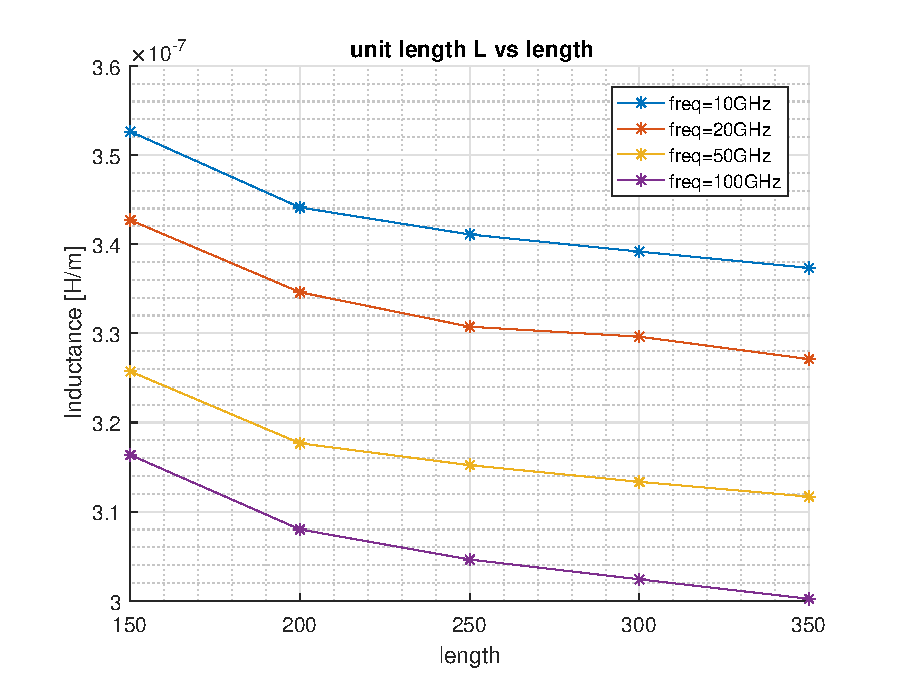
\includegraphics[width=7cm]{L_unit_len.eps}\label{fig:unit_L}}
  \vspace{0.5cm}
  \centering
   \caption{不同长度的CPW计算得到其单位长度RL值 \protect \\(CPW S=4um W=4um L=150um,200um,250um,300um,350um)} \label{fig:unit_RL2}
\end{figure}

为了得到模型本身的特性参数,需要去除端口效应的影响,基于此提出包含端口影响的等效电路模型,
如图\ref{fig:port},端口效应用串联R-L电路等效。R,L,G,C为无端口效应模型的本征参数,
$R_f$,$L_f$为端口效应电阻电感。按照图\ref{fig:port}端口效应对模型单位长度G、C没有影响,只对模型单位长度R、L的提取有影响。
\begin{figure}
  \centering
  \includegraphics[width=12cm]{port_influence.pdf}
  \caption{含端口效应的等效电路模型}\label{fig:port}
\end{figure}

以$R_t,L_t,G_t,C_t$,为模型总电阻、电感、电导、电容,有如下关系:
\begin{align}
  R_t &=R*len+2R_f  \label{equ:port_r}\\
  L_t &=L*len+2L_f \label{equ:port_l} \\
  G_t &=G*len  \label{equ:port_G}\\
  C_t &=C*len \label{equ:port_c}
\end{align}
   式\ref{equ:port_r}-- 式\ref{equ:port_c} 可转换为如下关系:
\begin{align}
  \frac{R_t}{len}&= R+\frac{2R_f}{len} \label{equ:port_r_new}\\
   \frac{L_t}{len}&= L+\frac{2L_f}{len} \label{equ:port_l_new} \\
   \frac{G_t}{len}&= G \label{equ:port_g_new} \\
  \frac{C_t}{len}&= C \label{equ:port_c_new}
\end{align}

从式\ref{equ:port_r_new}--式 \ref{equ:port_l_new}基于此端口效应模型可得到图\label{fig:unit_RL}所示结果,由于端口效应影响,
单位长度电阻、电感随着模型长度增加而减小。
\par
基于此端口效应模型以$1/len$为自变量,$R_t/len$为因变量做图,如图 2.4所示。
\begin{figure}[htb]\label{fig:1unit_RL}
\centering
  % Requires \usepackage{graphicx}
  \subfloat[单位长度R]{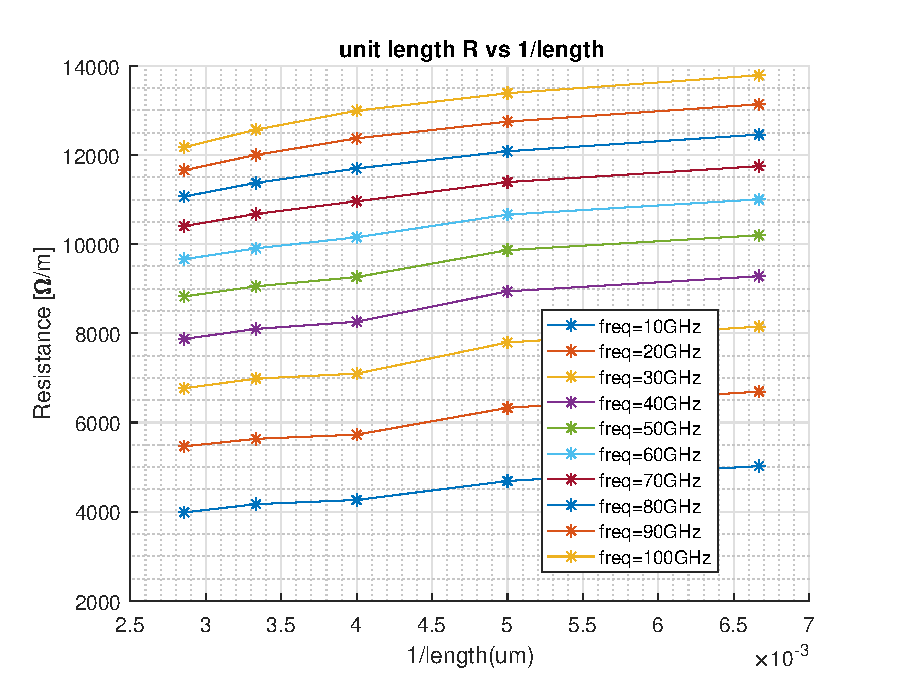
\includegraphics[width=7cm]{R_1unit_len.eps}\label{fig:1unit_R}}
 \hspace{0.1cm}
 %\qquad
  \subfloat[单位长度L]{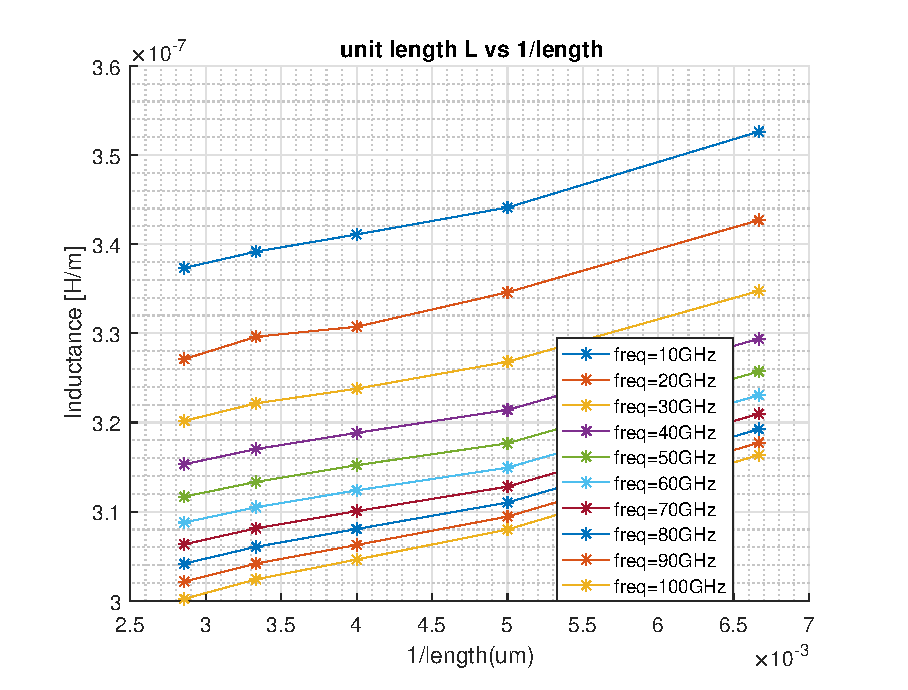
\includegraphics[width=7cm]{L_1unit_len.eps}\label{fig:1unit_L}}
  \vspace{0.5cm}
  \centering
   \caption{CPW模型单位长度电阻电感与模型长度的倒数的关系\protect \\(CPW S=4um W=4um L=150um,200um,250um,300um,350um)}
\end{figure}

结合式\ref{equ:port_r_new}--式 \ref{equ:port_l_new},通过最小二乘法做拟合直线,可提取模型本征单位长度\mbox{R、L}。

